\section{Интерференционные явления}


На любом приемнике получаем
\begin{equation*}
    \langle f\rangle = \frac{1}{\tau} \int_0^{\tau} f(t) \d t,
    \hspace{1 cm}
    \tau \gg T.
\end{equation*}
На деле фиксируем
\begin{equation*}
    I = \langle | \vc{S} | \rangle = \frac{c}{4\pi} \left[\vc{E}, \vc{H} \right] =
    \frac{c}{4\pi} \sqrt{\varepsilon} \langle E^2\rangle \sim \langle E^2\rangle.
\end{equation*}
Не стоит забывать, что
\begin{equation*}
    I = |E^2| = \langle (\vc{E} \cdot \vc{E}^*)\rangle_t.
\end{equation*}
Теперь, возвращаясь к интерференции,
\begin{equation*}
    \vc{E} = \vc{E}_1 + \vc{E}_2,
    \hspace{0.5cm} \Rightarrow \hspace{0.5cm}
    |\vc{E}^2| = |\vc{E}_1|^2 + |\vc{E}_2|^2 + (\vc{E}_1 \cdot \vc{E}_2^*) + (\vc{E}^*_1, \vc{E}_2).
\end{equation*}
Дальше вспоминаем про монохроматичность света
\begin{align*}
    \vc{E}_1 &= \vc{E}_{10} \exp \left(
        - i \omega_1 t + i k_1 l_1
    \right) \\
    \vc{E}_2 = \vc{E}_{20} \exp\left(
        - i \omega_2 t + i k_2 l_2
    \right)
\end{align*}
что приводит к
\begin{align*}
    I = |\vc{E}|^2 &= I_1 + I_2 + \left(\vc{E}_{10} \cdot \vc{E}_{20}\right) \cdot \left[
        \exp (i (\omega_2 - \omega_1)t + i (k_1 l_1 -k_2 l_2)) + \text{\ к.с.}
    \right] \\
    &= I_1 + I_2 + \left(\vc{E}_{10} \cdot \vc{E}_{20}\right) \cos\left(
        (\omega_2 - \omega_1) t + (k_1 l_1 - k_2 l_2)
    \right).
\end{align*}
Тогда для наблюдени интерференции хочется, чтобы

$\left(\vc{E}_{10} \cdot \vc{E}_{20}\right) \neq 0$ 

$\varphi_1(t) - \varphi_2 (t) = \const$

$\omega_1 = \omega_2$ 

\noindent
Однако хочется рассмотреть ситуацию

$\vc{E}_{10} \parallel \vc{E}_{20}$ 

$\varphi_1(t) - \varphi_2 (t) = 0$

$\omega_1 \approx \omega_2$

\noindent
В таком случае уравнение примет вид
\begin{align*}
    I = I_0 + I_0 + 2 I_0 \cos \left(
        (\omega_1 - \omega_2) t + \const
    \right) = 2 I_0 (1 + \cos((\omega_1 - \omega_2)t + \const)
\end{align*}
% Считая
% \begin{equation*}
%     T = \frac{2\pi}{\omega_1 - \omega_2} > \tau.
% \end{equation*}
% Так приходим к разрешающей способности спектральных приборов
% \begin{equation*}
%     R = \frac{\lambda}{\d \lambda} = \frac{\nu}{\d \nu}  \overset{\mathrm{exm}}{=} \frac{5893}{6}
% \end{equation*}
% для натрия. 
Вообще этот метод называется \textbf{гетероденирование} света. Нелинейной частью схемы является сам факт детектирования интенсивности. 
% https://ufn.ru/ufn56/ufn56_7/Russian/r567d.pdf
% см Ахманова никитина

% если у человека беда со слухом, то
%  демтрёдер -- лазерная спектроскопия
% 





\subsection{Фурье-спектроскопия}


\textbf{Пример из общей физики}. 
% % См. рис. О5.1, верно, что
Рассмотрим интерферометр Майкельсона. Движущееся зеркало испытывает доплеровский сдвиг при отражении:
\begin{equation*}
   \Delta \omega = \omega   -\omega' = \frac{v}{c}\omega.
\end{equation*}
Считая рахность фаз равной $\delta = (2\pi/\lambda) \Delta s$. Далее считаем
\begin{equation*}
    \bar{I} \sim (1 + e^{i \delta})(1 + e^{-i\delta}) \sim \frac{1}{2} \bar{I}_0 (1 + \cos \delta).
\end{equation*}
Куда уже подставляем $\Delta s = \Delta s_0 + 2 v t$, считая $\Delta s_0 = 0$:
\begin{equation*}
    I = 2 I_0 (1 + \cos (k \Delta)) = 2 I_0 \left( 1 + \cos \left(
            \frac{\omega}{c} v t
        \right)\right),
        \hspace{0.5cm} \Rightarrow \hspace{0.5cm}
        \Delta \omega = \omega \frac{v}{c}.
\end{equation*}
% Вообще надо аккуратно посчитать, но получится точно так. 
% сдвигаем неспеша

\textbf{Не монохроматическая волна}
Пусть есть некоторый сигнал с шириной линии $\delta k$, средней $K_0$ и
\begin{equation*}
    I = J_0 \delta K.
\end{equation*}
Выделим конкретную ширину $d k$ и $J_0 \d k$, тогда
\begin{equation*}
    \d I =2 J_0 \d k (1 + \cos (k \Delta)),
\end{equation*}
как в предыдущем примере. Приходим к интегралу
\begin{equation*}
    I = \int_{k_0-\delta k/2}^{k_0 + \delta k /2} 
    2 J_0 (1 + \cos(k \Delta)) \d k = 
    2 I_0 \left(1 + \cos\left( k \Delta\right) \ \text{sinc} \left(\frac{\delta k \Delta}{2}\right)\right)
\end{equation*}
где мы складываем интенсивности в силу приличности размерном ширины $\delta k$.
При этом \textit{видность}
\begin{equation*}
    V = \bigg| \text{sinc} \left(
        \frac{\delta k \Delta}{2}
    \right)
    \bigg|
\end{equation*}

\textbf{Фурье спектрометр}. Это как интерферометр Майкельсона, только двигается одно из зеркал. Интенсивность источника
\begin{equation*}
    I(\Delta) = 
    2 \int_0^\infty
    J(k) (1 + \cos k \Delta) \d k = 
    2 \int_0^{\infty} J(k) \d k + 
    2 \int_0^\infty 
    J(k) \cos (k \Delta) \d,
\end{equation*}
где первый интеграл равен $I(0)/2$, тогда
\begin{equation*}
    I(\Delta) - \frac{I(0)}{2} = 2 \int_0^{\infty} J(k) \cos (k \Delta) \d k.
\end{equation*}
То есть мы измерили в нуле, где-то далеко, делаем \textit{обратное преобразование Фурье} и находим $J(k)$.
% Должно получится что-то вроде
% \begin{equation*}
%     I(\Delta) - \frac{I(0)}{2} = \frac{1}{1+\frac{\Delta^2}{\Delta^2_0}}.
% \end{equation*}


\subsection{Многолучевая интерференция}


\textbf{Прошедшая волна}. Рассмотрим интерференцию на пластинке с показателем преломления $n$, толщиной $d$. Пусть свет монохроматичен,
пусть интенсивность света $I_0$.


Обозначим через $R$ коэффицент отражение света от границы раздела пластинки с воздухом. При отсутсвии поглощения $(1-R)$ проходит через границу, если среды по обе стороны одинаковы, то и $R$ будут одинаковы.  Тогда интенсивности прошедших пучков будут
\begin{equation*}
    I_{1'} = (1-R)^2, \hspace{5 mm} 
    I_{2'} = R^2(1-R)^2 I_0, \hspace{5 mm} 
    I_{3'} = R^4 (1-R)^2 I_0, \hspace{5 mm}  \ldots
\end{equation*}
а соответсвеющие вещественные амплитуды
\begin{equation*}
    a_{1'} = (1-R) a_0, \hspace{5 mm} 
    a_{2'} = R(1-R) a_0, \hspace{5 mm} 
    a_{3'} = R^2(1-R) a_0, \ldots .
\end{equation*}
Амплитула прошедшей волны представится убывающей геометрической прогрессией
\begin{equation*}
    \sub{a}{d} = a_0 (1-R)\left[1 + R e^{-i \Phi} + R^2 e^{-2i \Phi} + \ldots\right],
    \hspace{5 mm} 
    \Phi = k \Delta = \frac{4 \pi}{\lambda} n d \cos \psi,
    \hspace{0.5cm} \Rightarrow \hspace{0.5cm}
    \sub{a}{d} = \frac{1-R}{1-R e^{-i\Phi}} a_0.
\end{equation*}
где $\Phi$ -- разность фаз между соседними пучками.  Интенсивность прошедшей волны
\begin{equation*}
    \sub{I}{d} = \frac{(1-R)^2}{|1-R e^{-i \Phi}|^2} a_0^2 = \frac{(1-R)^2}{(1-R)^2 + 4 R \sin^2 (\Phi/2)} I_0,
\end{equation*}
что позволяет сделать некоторые выводы. 



\textbf{Отраженная волна}. Аналогичный расчёт приведет к
\begin{align*}
    &I_1 = R I_0, 
    &I_2 = R(1-R)^2 I_0, 
    &&I_3 = R^3 (1-R)^2 I_0, 
    &&\ldots, \\ 
    &a_1 = \sqrt{R} a_0, 
    &a_2 = - \sqrt{R} (1-R) a_0, 
    &&a_3 = - \sqrt{R} R (1-R) a_0, 
    &&\ldots,
\end{align*}
где знак в $a$ -- следставие появления $\lambda/2$. Резуьтирующая амплитуда будет иметь вид
\begin{equation*}
    a_r = \sqrt{R} a_0 - \sqrt{R} (1-R) a_0 e^{-i \Phi} \left[
        1 + R e^{- i \Phi} + R^2 e^{-2i \Phi} + \ldots
    \right],
    \hspace{0.5cm} \Rightarrow \hspace{0.5cm}
    I_r = \frac{4 R \sin^2 (\Phi/2)}{(1-R)^2 + 4 R \sin^2(\Phi/2)} I_0, 
\end{equation*}
где всё также $\Phi = k \Delta = \frac{4 \pi}{\lambda} n d \cos \psi$.


При $R \ll 1$ увидим случай двулучевой интерференции, при $R \approx 1$ уже интереснее (рис. \ref{fig:piks}). 
\begin{figure}[ht]
    \centering
    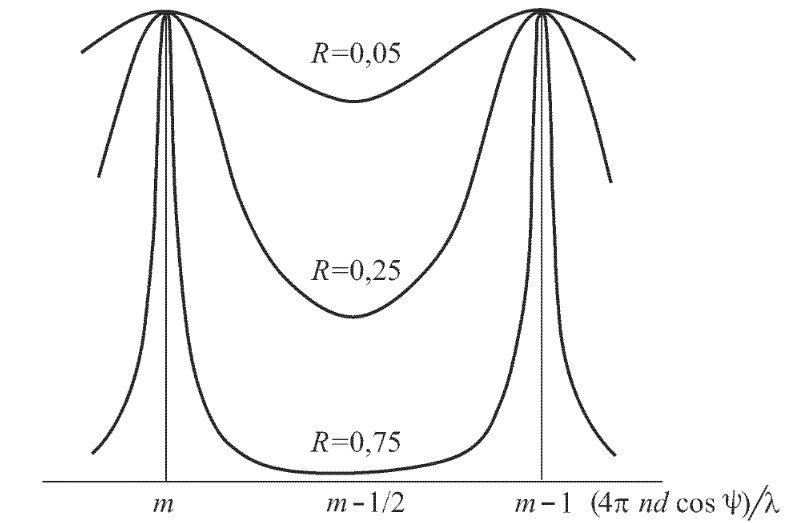
\includegraphics[width=0.3\textwidth]{figures/36_1.png}
    \caption{Пики для пластинки}
    \label{fig:piks}
\end{figure}
В окрестности максимума $m$-го порядка $\Phi = \pi m + \varphi$, тогда ввиду малости $\varphi$ можем написать
\begin{equation*}
    \sub{I}{d} = \frac{I_{\text{max}}}{1 + R \varphi^2/(1-R^2)},
    \hspace{0.5cm}
    \frac{R \varphi^2}{(1-R)^2} = 1 \text{ при } \sub{I}{d}= \frc{1}{2} \sub{I}{max},
    \hspace{0.5cm} \Rightarrow \hspace{0.5cm}
    \Delta \Phi = 2 \varphi = 2 \frac{1-R}{\sqrt{R}}.
\end{equation*}




\subsection{Интерферометр Фабри-Перо}

Рассмотрим пластинку с показателем $n$ на которую падает плоский фронт.
\begin{equation*}
    E_{\textnormal{out}} = E_0 \tau^2 + E_0 \tau^2 r^2 e^{i k \Delta} + 
    E_0 \tau^2 r^4 e^{2ik \Delta} + \ldots
\end{equation*}
Аккуратно считаем разность хода
\begin{equation*}
    n (AB + BC) - CD = 2 n h \cos \theta'.
\end{equation*}
Собираем всё вместе, и находим
\begin{equation*}
    E_{\textnormal{out}} = E_0 \tau^2 (1 + r^2 e^{ik\Delta} + r^4 e^{2ik \Delta}) = 
    \frac{E_0 \tau^2}{1-r^2 e^{ikD}}.
\end{equation*}
Теперь найдем интенсивность
\begin{equation*}
    I = E E^* = \frac{E_0^2 \tau^4}{(10r^2 e^{ik\delta})(1-r^2 e^{-ik\delta})} = 
    \frac{E_0^2 \tau^4}{1 + r^4 - 2 r^2 \cos (k \Delta)},
    \hspace{0.5cm} \Rightarrow \hspace{0.5cm}
    I_{\textnormal{max}} = E_0^2 \frac{\tau^4}{(1-r^2)^2}
\end{equation*}
вообще там $\tau_1$ и $\tau_2$, но всё хорошо, более того $1-r^2 \neq \tau^2$% \footnote{Проботать.}
, но приходим к $I_{\textnormal{max}} = E_0^2$ при $k \Delta = 2 \pi m$.
\begin{equation*}
    \Delta_m = \frac{2\pi m}{k} = m \lambda.
\end{equation*}
Стандратное значение $r = 0.04$.
% Можем получить колечки если пучок расходящийся.
% советуют сделать фабри перо лабу

\subsection{Равноотстоящие частоты}

Пусть есть некоторый набор частот
\begin{equation*}
    \nu_m = \nu_0 + m \Delta \nu.
    \hspace{1 cm} m \in [-l, l], \hspace{1 cm} 2l + 1 \text{\ частота всего.}
\end{equation*}
Эквидистантный (периодический) набор частот приведет к
\begin{equation*}
    E(t) = \sum_{m=-l}^l E_0 \exp\left(
        2 \pi i (\nu_0 + m \Delta \nu) t
    \right) = E e^{i 2 \pi \nu_0 t} \sum_{m=-l}^{l} \exp\left(
        2 \pi i \Delta \nu t m
    \right) = E_0 e^{\varphi} \left(
        \frac{1-\exp(2 \pi i \Delta \nu t N)}{1 - \exp(2 \pi i \Delta \nu t)}
    \right),
\end{equation*}
где $\varphi = i 2 \pi \nu_0 t$ но не совсем. Вспоминаем, что
\begin{equation*}
    \frac{1 - e^{i \varphi}}{1 - e^{i \psi}} =  \ldots
    % \frac{e^{i\varphi/2}}{e^{i \psi /2}}
    % \frac{e^{-i\varphi/2}-e^{-i\varphi/2}}{e^{-i\psi/2}-e^{-i\psi/2}
\end{equation*}
получаем, что
\begin{equation*}
    E(t) = E_0 e^{i \psi} \frac{\sin(\pi \Delta \nu N y)}{\sin\left(
        \pi \Delta \nu t
    \right)}    
    \hspace{0.5cm} \Rightarrow \hspace{0.5cm}
    I(t) = E_0^2 \frac{\sin^2(\pi \Delta \nu N t)}{\sin^2 (\pi \Delta \nu t)}.
\end{equation*}
Максимумы соответствуют $\pi \Delta _m = \pi m$, или $t_m = m / (\Delta \nu)$. Также можем получить, что характерная величина  $\Delta t = 1 / (\Delta \nu N)$